\subsection{Normalization and Haar feature-based cascade classifier}
Preprocessing of the image is needed in order to have a good recognition. We'll use for this purpose equalized gray images to a better detection of faces during the normalization. We use a Haar features-based cascade to detect the face.
\begin{figure}[ht]
	\centering		
	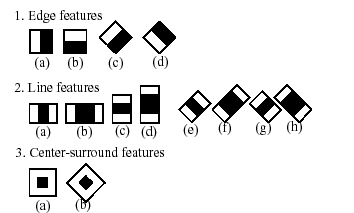
\includegraphics[width = 0.4\textwidth]{rsrc/Haarfeatures.png}
	\caption{Haar features used in openCV (including 45° features)}
	\label{fig:Haar features}
\end{figure}
The output will be the difference between the sum of the intensities on the whole picture and the intensities on the black part of the feature. The feature are scaled and move across the initial image. These are quickly calculated by using the corresponding intensity image.
\begin{figure}[ht]
	\centering		
	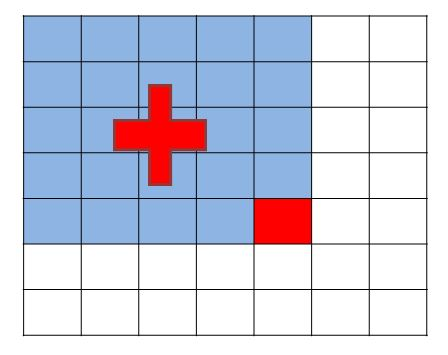
\includegraphics[width = 0.2\textwidth]{rsrc/IntegralImage.jpg}
	\caption{Integral image : sum of the intensities of the value of left and up pixels of the current pixel}
	\label{fig:Integral image}
\end{figure}
We use indeed two intensity images : one adding the left and up pixels of the analyzed pixel and an other intensity image adding the pixels in the corner of the current pixel made by two 45° lines.
The cascade is then trained. Adaboost is used for this purpose on positive images (a face, an eye, a nose, a mouth). The result is a sequences of criteria of recognition following a cascade checking of the object.
\begin{figure}[ht]
	\centering		
	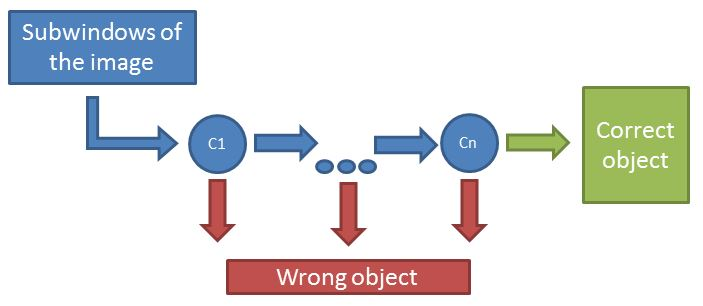
\includegraphics[width = 0.4\textwidth]{rsrc/Cascade.jpg}
	\caption{Cascade}
	\label{fig:Cascade}
\end{figure}
However, Haar will only recognize not rotated face. If we do not recognize a face, the face will be rotated and the same Haar process will be used. Once a face is detected we'll use again Haar features to detect the eyes or the mouth and nose. The angle remaining to have the eyes or nose and mouth aligned is then used to have these features aligned. The face is then cropped to the dimensions of the face detected by Haar features and resize to a specified size, so that every picture has the same size.

\subsection{Eigenfaces method}

The Eigenfaces method is based on a principal components analysis from a training set of images. To get those, each normalized image is translated into a vector. The principal components will be then determined : They have the highest eigenvalue in the diagonalized correlation matrix (made out of the image and the mean values of the training set). After selecting the principals components (first eigenvectors called eigenfaces in this case), each image can be then be approximated with those weighed eigenfaces :
\begin{equation}
x \approx  \hat{x} = \bar{x} + E_{x} * W \textrm{, where } 
\end{equation}
$x$ = vector representing the image,\\
$\hat{x}$ = approximated vector,\\
$\bar{x}$ = mean values of the vector during training,\\
$E_{x}$ = Matrix of eigenfaces (principal components),\\
$W$ = Matrix of weights of eigenfaces\\

$W$ is particular to each image and is calculated to minimize the distance between $x$ and $\bar{x}$:
\begin{equation}
W = E_{x}^T (x-\bar{x}) 
\end{equation}

The face recognized will be then the one in the training having its weight matrix $W$ the closest to the weight matrix of the current face analyzed. 

\subsection{Fisherfaces method}

The Fisherfaces method is an improved version of the Eigenfaces method that uses Linear Discriminant Analysis (LDA) rather than Principle Component Analysis (PCA) to find features that maximise the variance in the data. The problem with PCA is that it can consider variances in each picture, such as changing light sources as principle components and therefore not actually contain discriminating information about each face. To prevent this, Fisher's LDA method maximises the ratio of between-class scatter 
\begin{equation}
	\sum\limits_{i=1}^{c}N_{i}(\mu_{i}-\mu)(\mu_{i}-\mu)^T
\end{equation}
and within-class scatter.
\begin{equation}
	\sum\limits_{i=1}^{c}\sum\limits_{x_{j}\epsilon X_{i}}^{}(x_{j}-\mu_{i})(x_{j}-\mu_{i})^T
\end{equation}
Similar classes(faces) should therefore group together and dissimilar classes should be far away from each other.
Fisherfaces should produce lower errors than the Eigenfaces method and also be better at recognising faces in varying lighting conditions and different facial expressions.

\subsection{Local Binary Pattern Histogram}

The local binary pattern histogram method uses the local feature of the face. First, the image is sliced into squares.
To avoid problems of scale, The neighbours of a pixel analysed will be the ones on a circle with a varying radius and this pixel as center.
The intensity of the central pixel is then compared to the ones of its neighbours. (higher values become 1, lower ones become 0).
We then compute the new value of the central pixel, being the sum of powers of two combined with the value of neighbor taken clockwise. The point is to spot particular patterns of neighbor such as edges, lines, corner, flat areas.

\begin{figure}[ht]
\centering
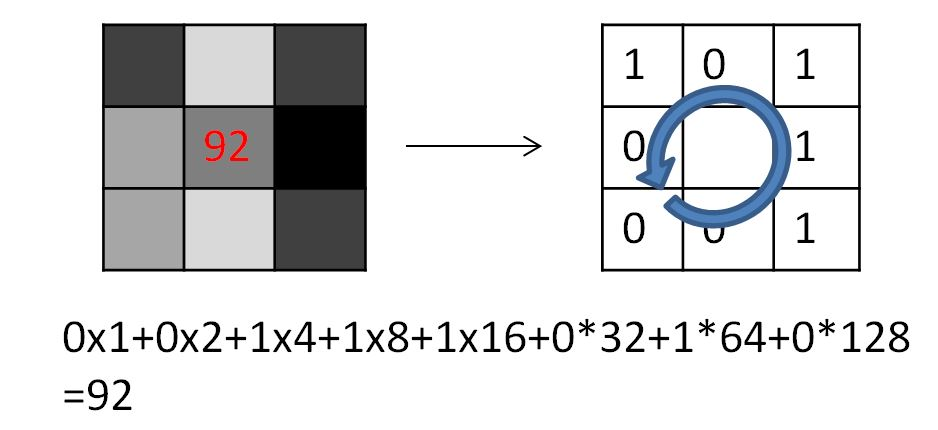
\includegraphics[width=2.5in]{rsrc/LBPH1.jpg}
\caption{Analysing the local structure}
\label{Local Structure}
\end{figure}

The histograms are then added (and not merged) for each part of the image. The resulting vector is then compared to the vectors obtained during the training. A fixed number of the closest vectors to the resulting vector is chosen and the person assigned to the greater number of these vector will be associated with the initial image.

\begin{figure}[ht]
\centering
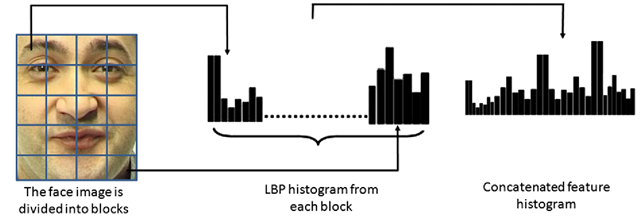
\includegraphics[width=2.5in]{rsrc/LBPH2.png}
\caption{Adding histograms (source : http://what-when-how.com/face-recognition/)}
\label{Adding histograms}
\end{figure}

\subsection{RBF and Convolutional NeuralNetwork}

NeuralNetwork stuff here
